\section{Problem Formulation}\label{sec:formulation}\label{sec:background}
\subsection{Merge Trees, Profiles, and Feature Identity}
For a sampled field $f_t$, the merge tree $T_t$ records sublevel components created at minima and joined at saddles; negating the field handles maxima~\cite{Tierny:2018:TTK}. Extraction and persistence simplification precede layout. A leaf $i$ has extremum location $p_i^t$ and support $S_i^t$, comprising the samples on its leaf arc. Augmented internal arcs retain samples for filling the profile. Write $h_t(v)$ for a node's scalar level and $\mathcal{D}_t(v)$ for its descendant leaves. The fixed-label merge matrix is
\begin{equation}\label{eq:merge}
V_{ij}^t=h_t(\lca(i,j)),\quad i\ne j;\qquad V_{ii}^t=f_t(p_i^t).
\end{equation}
Equal-level merges form one multifurcation. A one-dimensional profile $\psi_t$ places the extrema in leaf order $\pi_t$; the largest profile value between anchors $i,j$ gives their displayed merge level $V_{ij}^{\psi_t}$. Exact topology requires each strict subtree to form one contiguous block.

On a fixed grid, one-to-one Hungarian matching maximizes $|S_i^{t-1}\cap S_j^t|$ and discards zero-overlap pairs~\cite{STMTM:2026}. A matched leaf inherits its track identity; $\mu_t(i)$ denotes its predecessor. These links supply the temporal targets and motion samples below. The support is the leaf arc rather than the full component: internal arcs keep their own samples for reconstruction. Matching maximizes intersection counts, so a continuation is an assigned computational correspondence; unmatched leaves create or end tracks. A birth therefore contributes a current reference target but no predecessor target. The same matching is reused for every tested budget, keeping the temporal information fixed while the order constraints change.

\begin{figure}[!tb]
\centering
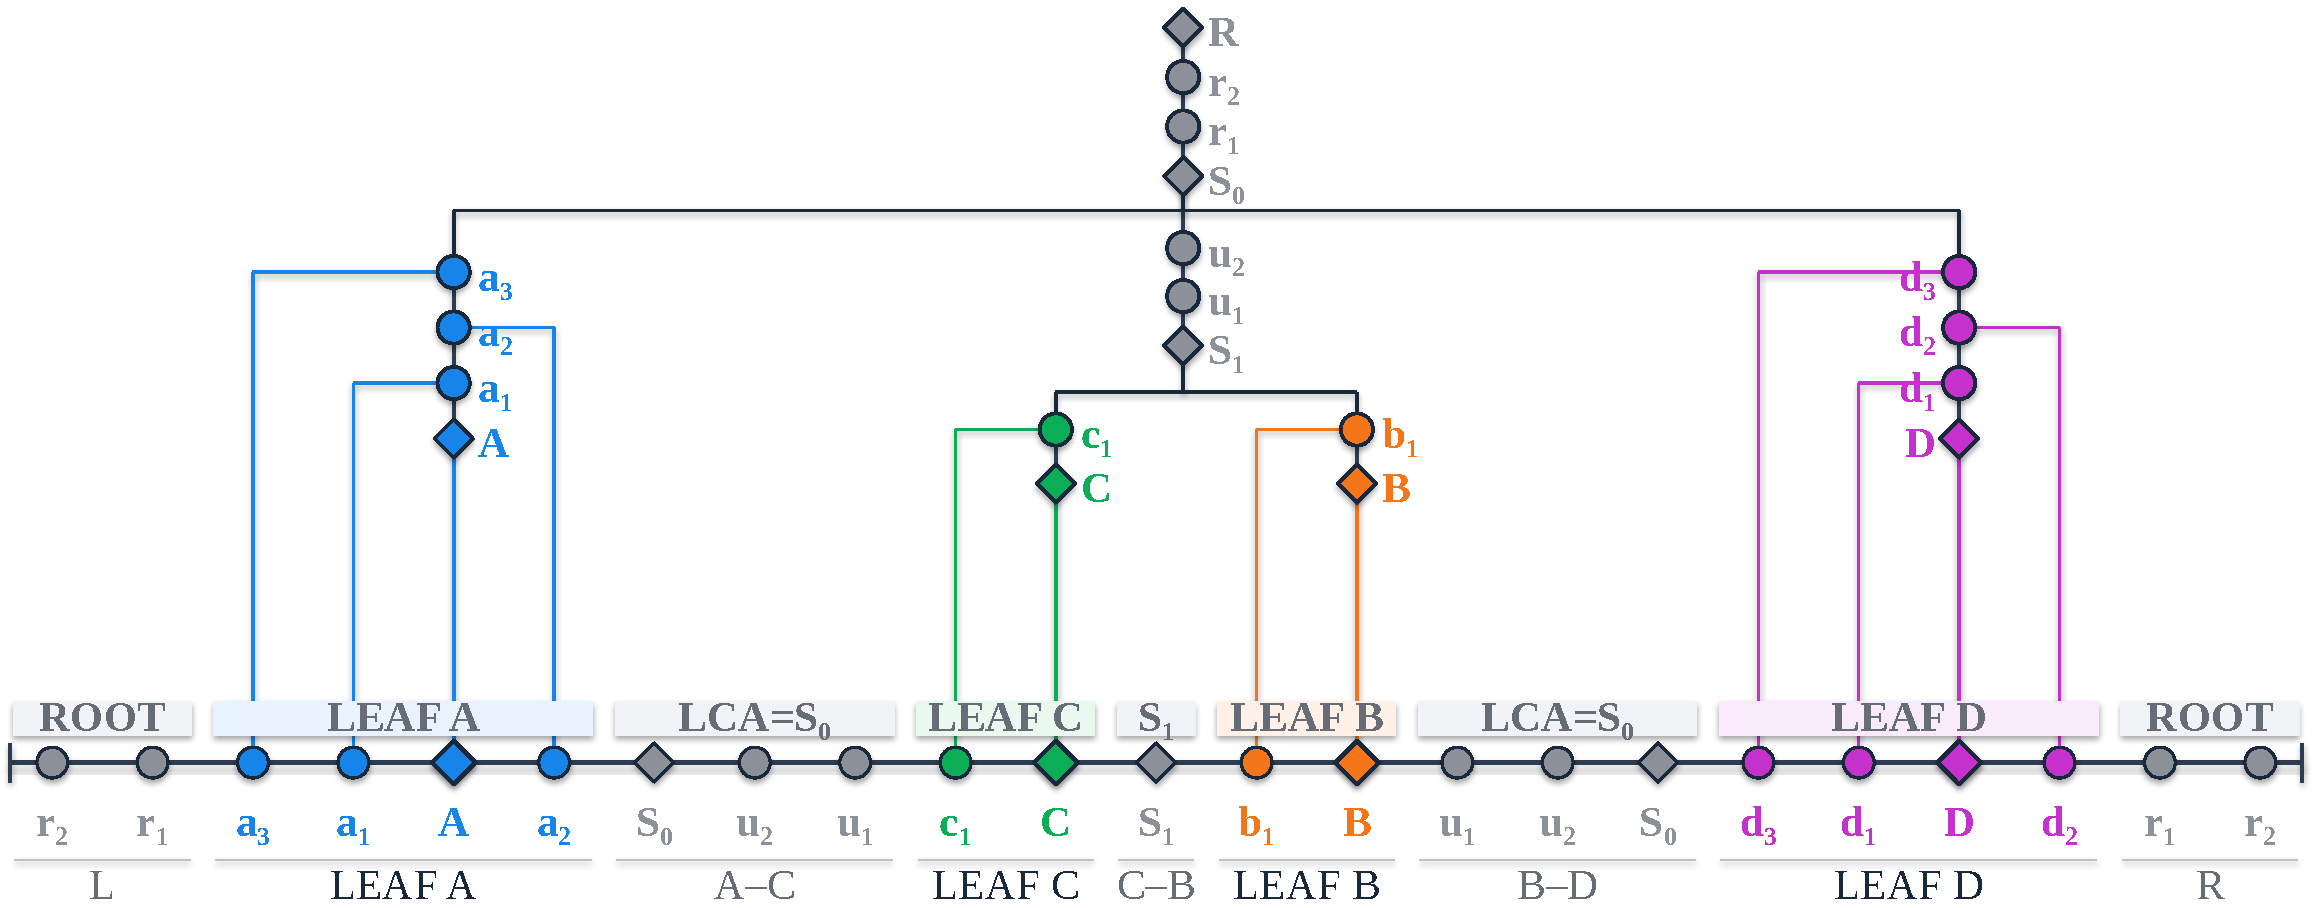
\includegraphics[width=\columnwidth]{figures/anchor_node_mapping.pdf}
\caption{An augmented merge tree and its profile retain the identities of extrema and regular arc samples. Their ordering makes every strict subtree contiguous.}
\label{fig:node-mapping}
\end{figure}
\subsection{Fixed Spatial Reference}\label{sec:reference-model}
\begin{figure}[!tb]
\centering
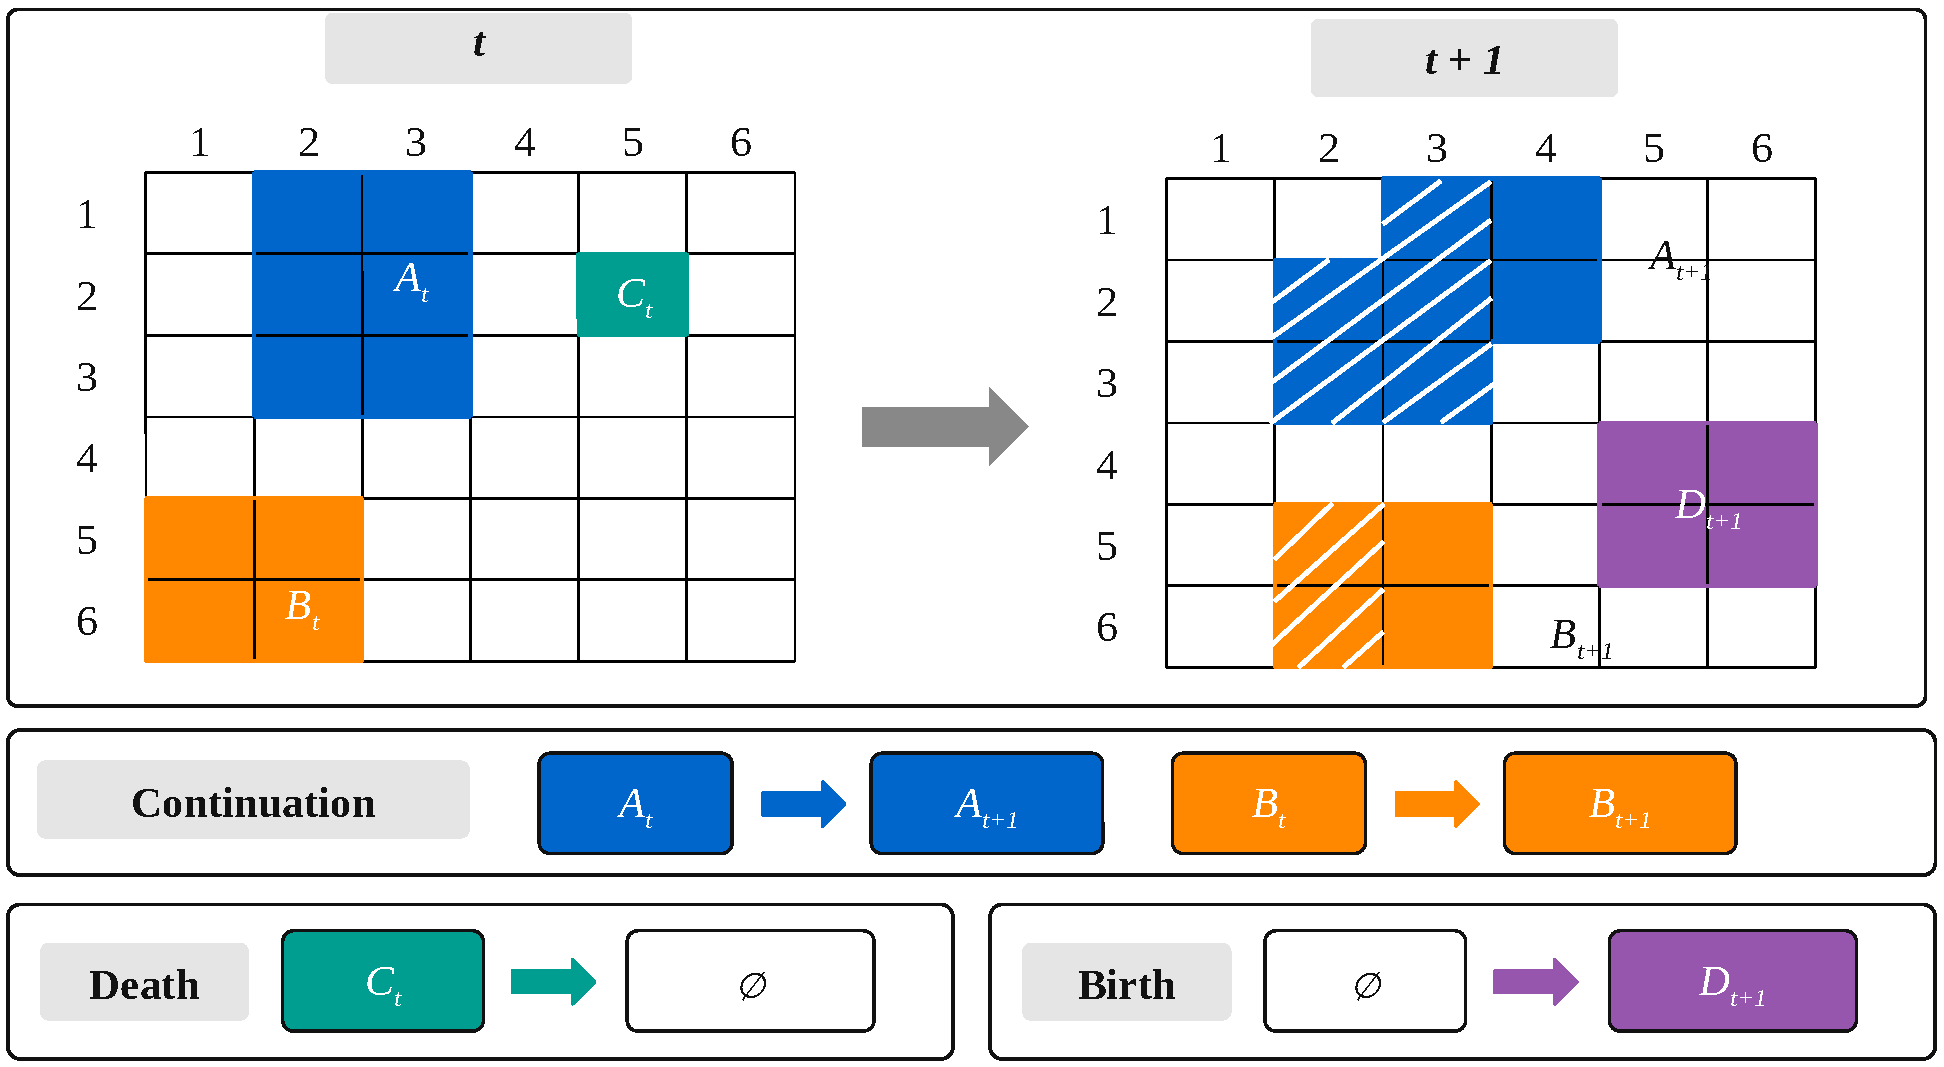
\includegraphics[width=\linewidth]{figures/anchor_leaf_correspondence.pdf}
\caption{Matching leaf-arc supports by one-to-one maximum overlap continues tracks across frames; unmatched leaves begin or end tracks. These correspondences supply the reference-motion samples.}
\label{fig:leaf_correspondence}
\end{figure}
The default direction maximizes squared matched-extremum motion:
\begin{equation}\label{eq:autodirection}
a^*\in\arg\max_{\|a\|=1}a^\top\Bigl(\sum_{t,i}\Delta p_i^t(\Delta p_i^t)^\top\Bigr)a,
\end{equation}
where $\Delta p_i^t=p_i^t-p_{\mu_t(i)}^{t-1}$ over valid links. Its sign makes total projected motion nonnegative; the longest domain axis handles zero motion energy. An analyst may supply a physical direction instead. For nearly zero signed motion, the largest-magnitude direction component is made positive; repeated leading eigenvalues can be resolved using a chosen physical axis. This separates reference estimation from the layout search: a budget changes the admissible map, while the coordinate being approximated stays fixed. Projected domain corners define one origin $o$ and extent $L$, giving
\begin{equation}\label{eq:reference}
q_i^t=\langle a^*,p_i^t\rangle-o\in[0,L].
\end{equation}
Direction, origin and extent remain fixed across frames and budgets. Relative geometry uses support-centroid distances $d_{ij}^t$; the targets $q_i^t$ use extremum locations. Thus support growth can change relative-distance terms without moving a feature's spatial target.

\subsection{A Unified Layout Formulation}\label{sec:common}
Each leaf occupies an interval of width $W_i=s\,m_i$ and center $z_i$, where $m_i$ is its support measure and $s$ is fixed. The layout set $\mathcal{L}(\pi;W)$ places these intervals in order $\pi$ inside $[0,L]$, with gap at least $g$ and anchor slack $|x_i-z_i|\le\rho W_i/2$. Two order costs distinguish point ordering from packing:
\begin{equation}\label{eq:nroe}
\begin{aligned}
\nroe(\pi)&=\frac{\max_{j\le k}[q_{\pi(j)}-q_{\pi(k)}]^+}{2L},\\
\tau(\pi)&=\min_{(x,z)\in\mathcal{L}(\pi;W)}\|x-q\|_\infty .
\end{aligned}
\end{equation}
NROE is the least normalized worst displacement of points in order $\pi$; $\tau$ includes the intervals and is an exactly solvable minimax linear program. Merge error measures the displayed hierarchy:
\begin{equation}\label{eq:dtop}
\dtop(\psi,T)=\max_{i,j}|V_{ij}^{\psi}-V_{ij}|\le\eta.
\end{equation}
The diagonal includes extremum values. Under complete fixed labelling this cophenetic error equals labelled interleaving distance and bounds the unlabelled interleaving and bottleneck distances~\cite{Munch:2019:LINF,Gasparovic:2024:IID,Morozov:2013:IDMT}.

These variables separate layout priorities in the common model
\begin{equation}\label{eq:family}
\begin{aligned}
\min_{\pi\in\Pi,\,(x,z)\in\mathcal{L}(\pi;W)}\;&\lambda_RE_R+\lambda_GE_G+\lambda_ME_M+\lambda_CE_C\\
\mathrm{s.t.}\;&\dtop\le\eta.
\end{aligned}
\end{equation}
where the terms fit spatial references, support distances, matched temporal targets and interval centers. TMTM packs tree-compatible blocks and aligns them by overlap; ST-MTM fits relative geometry with temporal constraints. Both preserve the tree and have no absolute-reference penalty. Anchoring adds $E_R$. \subsection{Conflict Between Topology and Spatial Position}
A projection can follow every $q_i$, but the order $A,C,D,B$ breaks the $A,B$ subtree block. The issue is the interaction between the spatial target order and the contiguous blocks required by a profile. Keeping those blocks may displace anchors; allowing some merge-level error may admit an order closer to the targets. This structural conflict precedes any choice of optimizer.

We address three questions: how much displacement exact topology forces (RQ1), how finite feature widths and interval constraints increase that cost (RQ2), and which conflicts can be released by bounded merge-level error (RQ3). The next section answers them in this order; the construction then uses the same quantities to select and place a map.
